\newpage
\section{Описание структуры компилятора}

Общая схема работы готового продукта «Компилятор» представляется следующим образом: консольное приложение запускает внутри себя компоненты содержательных модулей, представленных на рисунке 1. В процессе анализируется файл исходного кода, строится синтаксическое дерево и другие промежуточные представления программы, и генерируется код на языке LLVM IR. Полученный файл может быть транслирован в объектный с помощью утилиты LLCompiler (llc) и в дальнейшем может быть использован компоновщиком для получения исполняемого файла.

\begin{figure}[h]
    \centering
    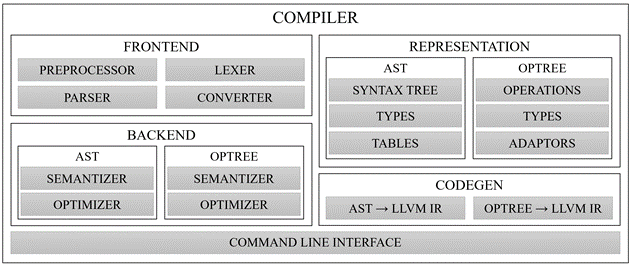
\includegraphics[width=\textwidth]{images/project-structure.png}
    \caption{Структура проекта.}
\end{figure}

Для обеспечения корректности работы будет разработан комплект функциональных и интеграционных тестов для компонентов проекта.

Предполагается, что компилятор будет работать с Python-подобным статически типизированным языком, в котором будут присутствовать основные языковые конструкции (объявления функций и переменных, условия, циклы, вызовы функций, вычисление арифметико-логических выражений), возможность вывода текста на экран и считывания данных с клавиатуры.

В предлагаемой реализации компиляция кода должна осуществляться в несколько этапов. За каждый из этапов отвечает один из представленных в рамках проекта модулей, взаимодействующих подобно конвейеру: выходные данные одного этапа являются входными для следующего, как это видно на рисунке 2. В предыдущей работе, упомянутой ранее, анализ компилируемой программы производился с использованием синтаксического дерева, что отражено в левой части схемы. Теперь ему на смену пришло другое промежуточное представление – дерево операций, этапы анализа которого представлены справа.

\begin{figure}[h]
    \centering
    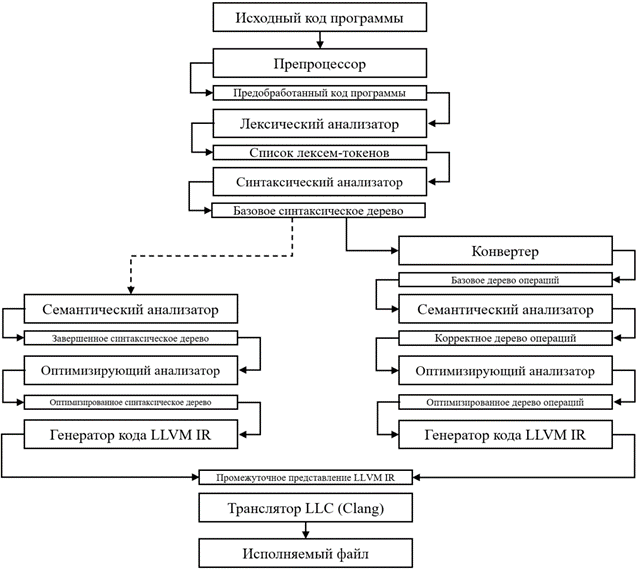
\includegraphics[width=\textwidth]{images/compilation-pipeline.png}
    \caption{Этапы компиляции.}
\end{figure}
